% !TEX root = main.tex

\section{半监督学习}
让学习器不与外界交互、自动利用未标记样本来提升学习性能就是半监督学习\footnote{如果是强化学习,则需要与外界进行交互获得反馈}。

\begin{figure}[H]
\centering
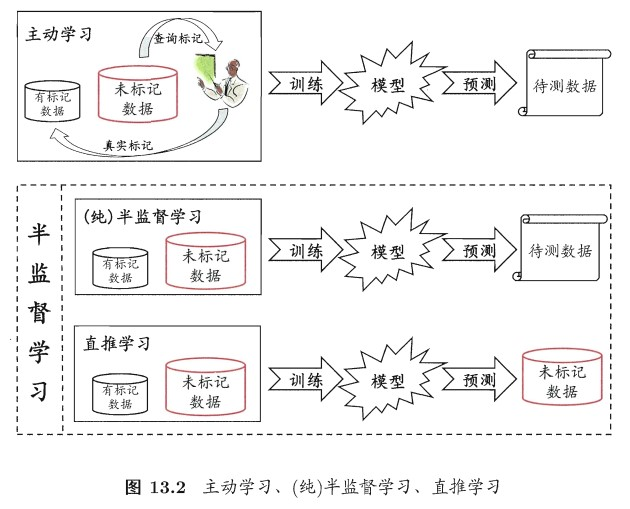
\includegraphics[width=0.8\linewidth]{fig/semi-supervised_learning.jpg}
\end{figure}

\subsection{生成式方法}
假设所有数据(无论是否有标记)都是由\textbf{同一个潜在的模型生成}的。

给定样本$\vx$,真实类别标记为$y\in\mY=\{1,2,\ldots,N\}$。
假设样本由高斯混合模型生成,且每个类别对应一个高斯混合成分,即数据样本基于以下概率密度生成
\[p(\vx)=\sum_{i=1}^N\alpha_i\cdot p(\vx\mid\vmu_i,\Sigma_i)\]
其中混合系数$\alpha_i\geq 0$,$\sum_{i=1}^N\alpha_i=1$。
$p(\vx\mid\vmu_i,\Sigma_i)$是样本$\vx$属于第$i$个高斯混合成分的概率,$\vmu_i$和$\Sigma_i$为该高斯混合成分的参数。

令$f(\vx)\in\mY$表示模型$f$对$\vx$的预测标记,$\Theta\in\{1,2,\ldots,N\}$表示样本$\vx$隶属的高斯混合成分。
最大化后验概率知
\[\begin{aligned}
f(\vx) &= \argmax_{j\in\mY}p(y=j\mid\vx)\\
&= \argmax_{j\in\mY}\sum_{i=1}^Np(y=j\mid\Theta=i,\vx)\cdot p(\Theta=i\mid\vx)
\end{aligned}\]
用极大似然法可以估计参数,并用EM算法求解。

此类方法简单、易于实现,在有标记数据极少的情形下往往比其他方法性能更好。
然而,此类方法有一个关键:模型假设必须准确,即假设的生成式模型必须与真实数据分布吻合;
否则利用未标记数据反而会显著降低泛化性能。

\subsection{半监督SVM}
半监督SVM(Semi-Supervised SVM, S3VM)是SVM在半监督学习上的推广。
S3VM试图找到能将两类有标记样本分开,且穿过数据低密度区域的划分超平面,采用的基本假设是低密度分隔(low-density separation)。

半监督SVM中最著名的是TSVM(Transductive SVM)。
TSVM试图考虑对未标记样本进行各种可能的标记指派,尝试将每个未标记样本分别作为正例或反例,然后再所有这些结果中,寻求一个在所有样本上间隔最大化的划分超平面。
一旦划分超平面得以确定,未标记样本的最终标记指派就是其预测结果。

TSVM采用局部搜索来迭代寻找近似解。
\begin{figure}[H]
\centering
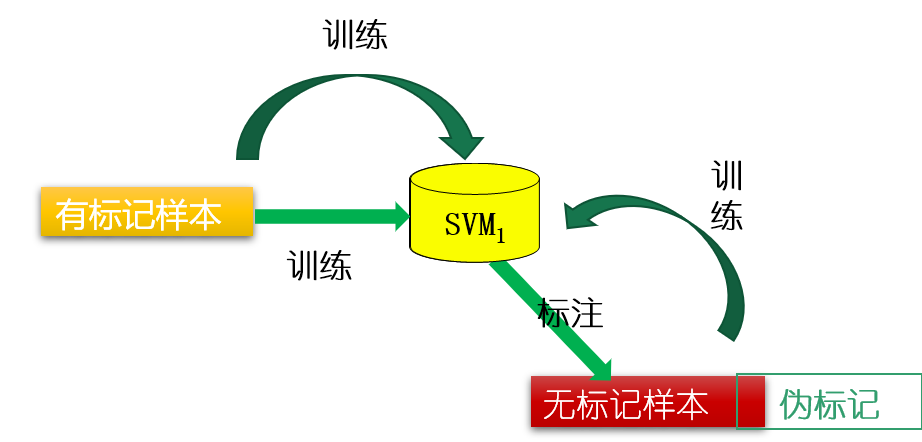
\includegraphics[width=0.6\linewidth]{fig/TSVM.png}
\end{figure}

未标记样本进行标记指派及调整的过程中,有可能出现类别不平衡问题,即某类的样本远多于另一类。
为了减轻类别不平衡性所造成的不利影响,可对算法稍加改进:将优化目标中的$C_u$项拆分为$C_u^+$与$C_u^-$两项,并在初始化时令$C_u^+=\frac{u_-}{u_+}C_u^-$。

\subsection{图半监督学习}
给定一个数据集,我们可将其映射为一个图,数据集中每个样本对应于图中一个结点,若两个样本之间的相似度/相关性很高,则对应的结点之间存在一条边,边的强度(strength)正比于样本之间的相似度/相关性。

我们可将有标记样本所对应的结点想象为染过色,而未标记样本所对应的结点则尚未染色。
于是,半监督学习就对应于“颜色”在图上扩散或传播的过程。

先基于标签数据与无标签数据的集合$D_l\cup D_u$建图$G=(V,E)$,其中结点集
\[V=\{\vx_1,\ldots,\vx_l,\vx_{l+1},\ldots,\vx_{l+u}\}\]
边集$E$可表示为一个亲和(affinity)矩阵,常基于高斯函数定义为
\[W_{ij}=\begin{cases}
\exp\lrp{\frac{-\norm{\vx_i-\vx_j}_2^2}{2\sigma^2}} & i\ne j\\
0 & \text{otherwise}
\end{cases}\]

相似的样本应具有相似的标记,即得到最优结果于是可定义关于$f$的能量函数(energy function)。

\subsection{半监督聚类}
聚类是一种典型的无监督学习任务,然而在现实聚类任务中我们往往能获得一些\textbf{额外的监督信息},于是可通过半监督聚类来利用监督信息以获得更好的聚类效果。

聚类任务中获得的监督信息大致有两种类型:
\begin{itemize}
\item 第一种类型是“必连”(must-link)与“勿连”(cannot-link)约束,前者是指样本必属于同一个簇,后者则是指样本必不属于同一个簇
\item 第二种类型的监督信息则是少量的有标记样本
\end{itemize}

约束k均值(Constrained k-means)算法[Wagstaff et al., 2001]是利用第一类监督信息的代表。
该算法是k均值算法的扩展,它在聚类过程中要确保“必连”关系集合与“勿连”关系集合中的约束得以满足,否则将返回错误提示。
不冲突则选择最近的簇,冲突则尝试次近的簇。

第二类监督信息可假设少量有标记样本属于$k$个聚类簇。
这样的监督信息利用起来很容易:直接将它们作为“种子”,用它们初始化$k$均值算法的$k$个聚类中心,并且在聚类簇迭代更新过程中\textbf{不改变}种子样本的簇隶属关系。
这样就得到了约束种子k均值(Constrained Seed k-means)算法[Basu et al., 2002]。